\documentclass[11pt]{article}
\usepackage[margin = 1in]{geometry}
\usepackage{amsmath}
\usepackage{amssymb}
\usepackage{amsthm}
\usepackage{graphicx}
\usepackage{subfig}
\usepackage{enumitem}
\usepackage{url}
\usepackage{pdfpages}
\usepackage{listings}
\usepackage[parfill]{parskip}
\newcommand{\skipline}{\vspace{\baselineskip}}
\newenvironment{problem}[1]{\textbf{Problem #1: }}{\newpage}


\begin{document}
	\includepdf{GradingSheet}
	\begin{center}
		\textbf{Homework 2} \\
		\textbf{Computer Vision} \\
		\textbf{CS 559} \\
		\textbf{Stephen Giang RedID: 823184070} \\
	\end{center}
	\skipline 

	\begin{problem}{1}
		Explain conditions under which the use of a lookup table (LUT), instead of calculating the mapping pixel by pixel, reduces the computation.  Express the conditions in terms of number of graylevels $L$ and resolution $n$. 
		\\ \\
		Notice the following:
		\\ \\
		Calculating the mapping pixel by pixel would force us to traverse through every pixel and apply the mapping calculating a total of $n^2$ times (that is for a square n $\times$ n image).
		\\ \\
		With the use of the lookup table, we know the following: $0 \leq f(x,y) < L$.  This means we can make a table with $L$ elements, each element being the mapping calculation of each grayscale levels to the new outputted grayscale level.  Now that all the calculations are done, we use the table to assign each pixel value from the original image to the new image. This means we only need to do $L$ calculations and $n^2$ assignments.
		\\ \\
		If $n^2 > L$, we reduce the computation by $n^2 - L$ using the lookup table. 
		\\ \\ 
		If $n^2 = L$, then either method is just as good for computations.
		\\ \\
		If $n^2 < L$, then calculating the mapping pixel by pixel would be reduce the computations by $L - n^2$ computations. 
	\end{problem}

	\begin{problem}{2}
		Many (infinite number) of passes of contrast stretching with the mapping \\
		\[g = \begin{cases}
		0.4f & 0 \leq f \leq 119 \\
		f & 120 \leq f \leq 255
		\end{cases}\]
		is applied to a perfectly equalized 8-bit input image.  Draw and carefully label the normalized histogram 
		of the output image. 
		\\ \\
		Notice that if $f$ is a perfectly equalized 8-bit input image, then its histogram looks like the left histogram.  If we take our mapped image, we get the right histogram:
		\\ 
		\begin{figure}[h!]
			\includegraphics[width = 9cm]{Matlab/F2.eps}
			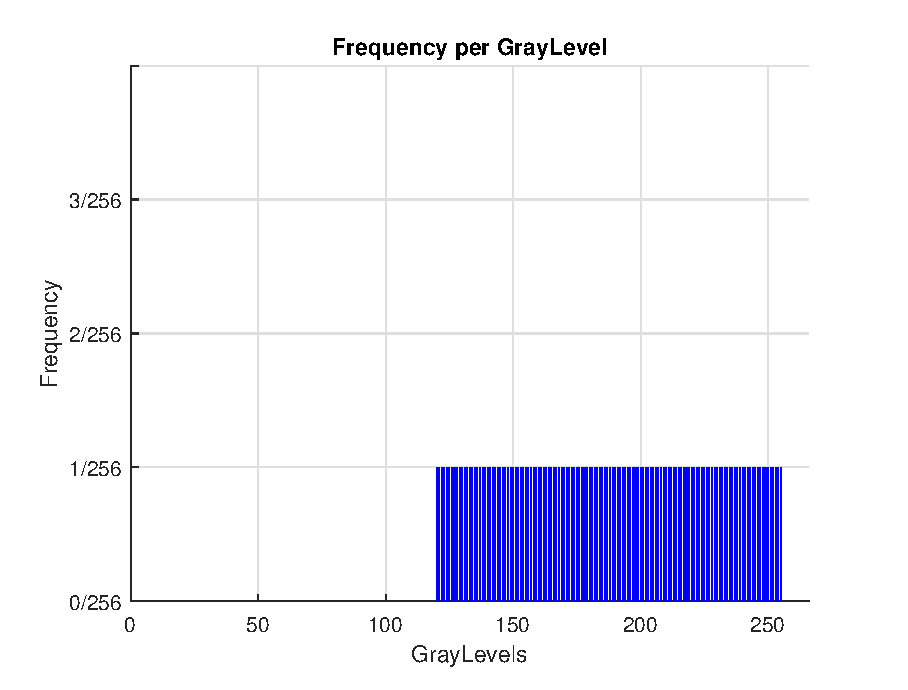
\includegraphics[width = 9cm]{Matlab/G2.eps}
		\end{figure}
		\\ \\
		Notice that with a perfectly equalized image, we get a flat histogram where there is an equal frequency with each graylevel, frequency being the probability of choosing a random pixel with a specific grayscale level.  Because of the floor function when multiplying by .4, if we do this an infinite number of times, we get that all grayscale levels goes to 0 for $0 < f \leq 119$.  This means that the frequency of 0  go to 120/L = 120/256. (There is a tiny bar over 0, that goes to 120/256 on the right histogram).
	\end{problem}

	\begin{problem}{3}
		An 8-bit image has a normalized histogram defined by
		\[h(l) = \begin{cases}
			\frac{1}{206} & 0 \leq l  < 100 \\
			\frac{1}{412} & 100 \leq l  < 200 \\
			\frac{1}{206} & 200 \leq l  < 256
		\end{cases}\]
		Suppose that each pixel is ANDed with 0100 0000, and is set to white if the result of ANDing is non-zero, otherwise is set to black if the result is zero (this operation is called bit-plane slicing). Draw and carefully label the normalized histogram of the resulting output image.
		\\ \\
		The conversion from grayscale level ($G$) to binary code ($B$) is found through the linear combination:
		\[ G = a(128) + b(64) + c(32) + d(16) + f(8) + h(4) + j(2) + k(1)\]
		where we have $a,b,c,d,f,h,j,k \in \{0,1\}$. From this, we get $B = a\,b\,c\,d\,f\,h\,j\,k$
		\\ \\ 
		For $B = a\,b\,c\,d\,f\,h\,j\,k$, notice that when ANDing with 0100 0000, we only get nonzero results when $b = 1$.  We get zero when $b = 0$.
		\begin{enumerate}[label = (\alph*)]
			\item For $0 \leq G < 64$, we get $b = 0$. 
			\item For $64 \leq G < 128$, we get $b = 1$. 
			\item For $128 \leq G < 192$, we get $b = 0$.
			\item For $192 \leq G < 256$, we get $b = 1$. 
		\end{enumerate}  
		Using the above results, we get that for greyscale values $0 \leq l < 100$, $64$ grayscale levels become 0 (Black).  For greyscale values $100 \leq l < 200$, $64$ grayscale levels become 0 (Black).  For greyscale values $200 \leq l < 256$, $0$ grayscale levels become 0 (Black).  From these results, we get the following frequencies:
		\begin{align*} 
			\text{Black Frequency} &= \frac{1}{206}(64) + \frac{1}{412}(64) + \frac{1}{256}(0) = \frac{96}{206} \\
			\text{White Frequency} &= 1 - \text{ Black Frequency } = 1 - \frac{96}{256} = \frac{110}{206}
		\end{align*} 
		\begin{figure}[h!]
			\includegraphics[width = 9cm, height = 6.25cm]{Matlab/H3.eps}
			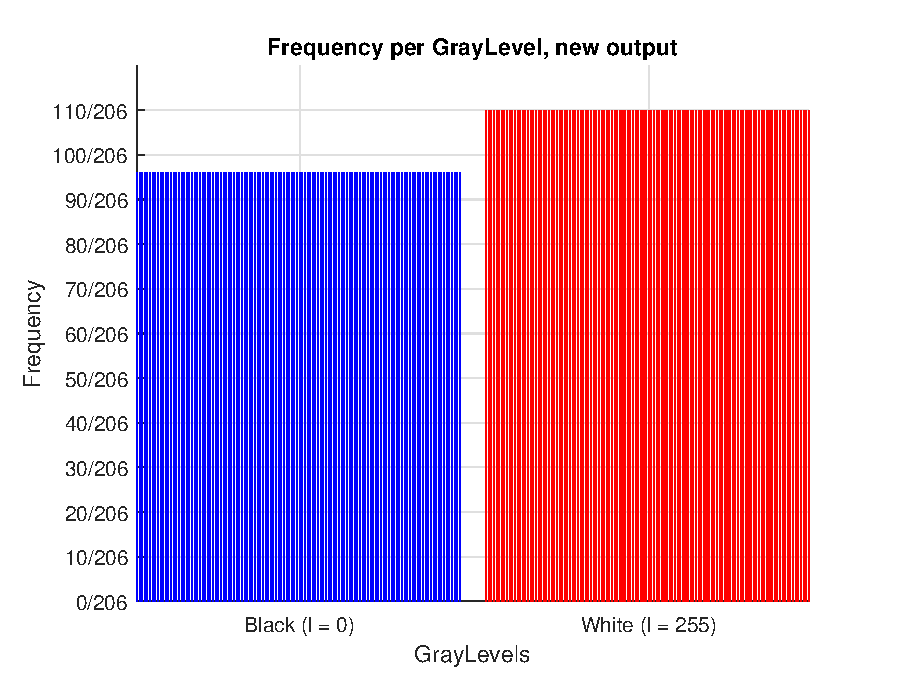
\includegraphics[width = 9cm, height = 6.25cm]{Matlab/G3.eps}
		\end{figure}
		
	\end{problem}
	
	\begin{problem}{4}
		The purpose of this assignment is for you to come up with a measure (formula, procedure, or algorithm) to determine the similarity between two color images, with 0 being completely difference and 100 being exactly the same. Explain why your measure is appropriate. Program your procedure and apply it to determine how similar each image B, C or D is similar to the image A. One method would be to compare the histogram of the images, but you can propose an alternative method of your own. I do not expect you to proposed a sophisticated measure, rather I want you to appreciate that images that are so easy for our eyes to identify their similarity and differences, are very difficult to do the same using computer vision. Note: Download this assignment, then open it, click on each image and save it as .jpg. 
		\\ \\
		\begin{figure}[h!]
			\includegraphics[width = 4cm, height = 4cm]{Photos/A.jpg}
			\includegraphics[width = 4cm, height = 4cm]{Photos/B.jpg}
			\includegraphics[width = 4cm, height = 4cm]{Photos/C.jpg}
			\includegraphics[width = 4cm, height = 4cm]{Photos/D.jpg}
		\end{figure}
		\\ 
		\text{} \hspace{1.5cm} (A) \hspace{3.25cm} (B) \hspace{3.5cm} (C) \hspace{3.25cm} (D)
		\\ \\
		For this program, what I did was I found the difference between image A and image B in RGB values at each pixel.  Then I divided each element by 255 to see a percent change.  From there, I added all the entries, and divided by the total number of entries. This gave me a difference average from pixel to pixel.  To find the similarity, its just (1 - average).
		\\ \\
		Notice my results:
		\begin{itemize}[label = -]
			\item Image A is about 100.00 \% the same as Image A 
			\item Image B is about 87.80 \% the same as Image A 
			\item Image C is about 96.90 \% the same as Image A 
			\item Image D is about 68.78 \% the same as Image A 
		\end{itemize}
		\includepdf{Matlab/similarPDF}
		\includepdf{Matlab/prob4PDF}
	\end{problem}

	\begin{problem}{5}
		Write a program in Python or Matlab that takes an RGB image of size W by H and an integer k and produces an output image of size kW by kH where k is an integer greater than one (sometime this is called resampling). The enlarged image must be in appearance as close as possible to the original image. Use bilinear interpolation or another technique of your choice.  Demonstrate your work by producing an input image and two output images one with k=2 and one with k=3.
		\\ \\
		For this program, what I did was I mapped each pixel (x,y) to (kx,ky).  Then for the pixels between (kx,ky) and (k(x+1),ky), I filled it in with a weighted average.  For example, for the set \{1 \underline{A} \underline{B} 4\}, I found that we can equally space each entry by a distance of $\frac{4-1}{3} = 1$.  Then I simply added each left entry with that distance to get equally spaces sets between (kx,ky) and (k(x+1),ky). From there, I did the same thing but column wise. 
		\\ \\
		Notice the images below with each photo being 1x, 2x, 3x respectively:
		\begin{figure}[h!]
			\centering
			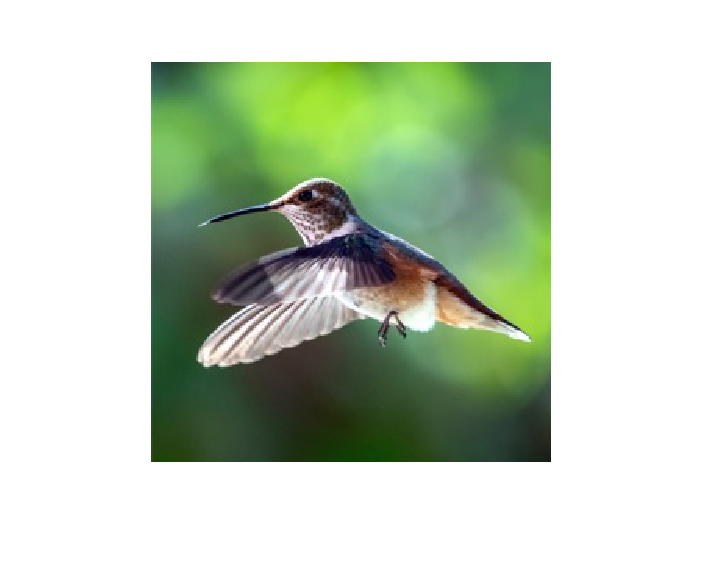
\includegraphics{Matlab/Bird1}
		\end{figure}
		\begin{figure}
			\centering
			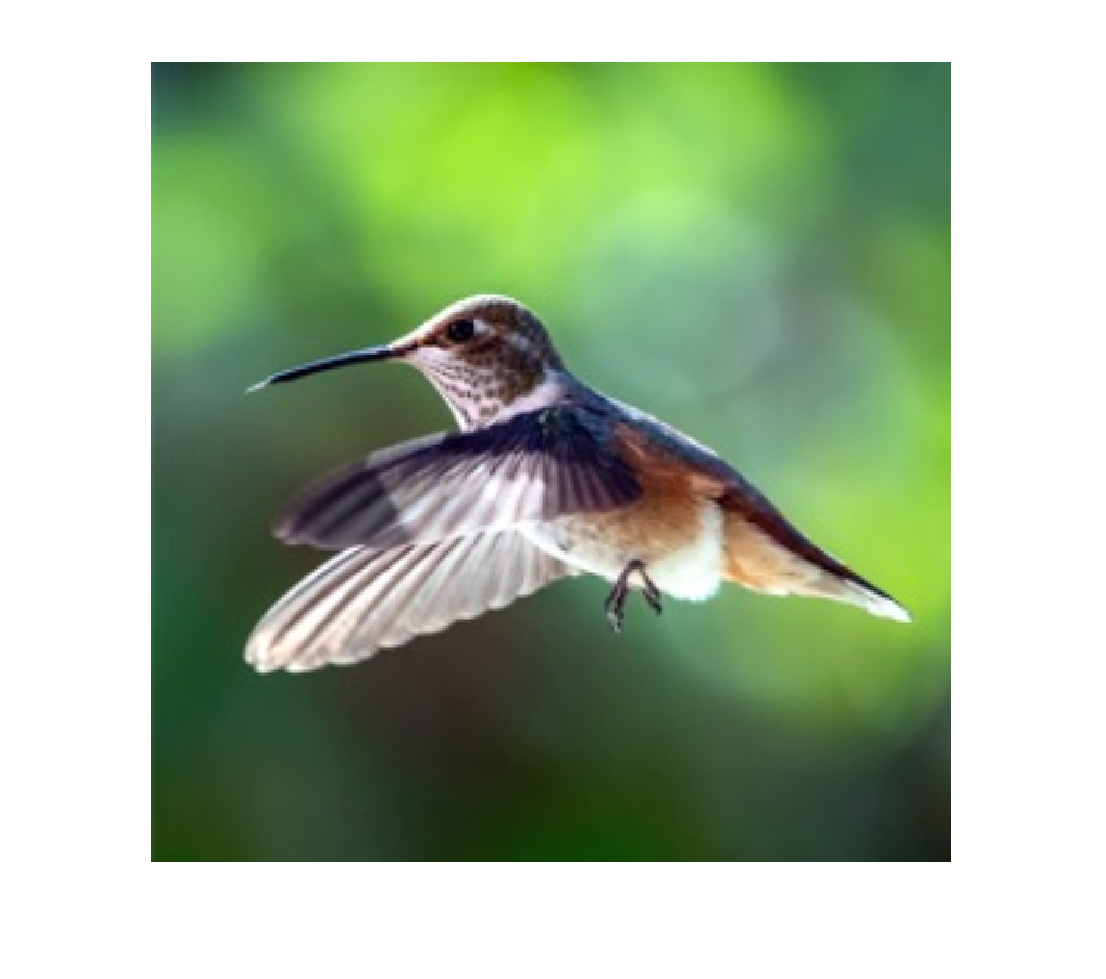
\includegraphics{Matlab/Bird2}
		\end{figure}
		\includepdf{Matlab/Bird3PDF}
		\includepdf[pages=1-]{Matlab/bilinearInterplPDF}
		\includepdf{Matlab/prob5PDF}
	\end{problem}


\end{document}
